
\section{Background}
\label{sec:Background}

In this section, we will present an introduction over the SMT problem solving. Later we will focus on the theory solver part.

\subsection{The SAT problem}
In classical propositional logic, a boolean formula is constructed from a set of variables connected by logical operators like \(\wedge, \vee, \neg\). The boolean variables can be assigned a truth value that is either  $\texttt{true}$ or  $\texttt{false}$. The classical $ SAT\ problem$is defined as, 
given a boolean formula, is there any assignment, such that the formula is evaluated to $\texttt{true}$. There are many decision procedures to solve this classic SAT problem. Among them, the DPLL \cite{dpll} procedure is  most frequently used in most modern SAT solvers. 

\subsection{The SMT Problem}
\label{sec:dpllt procedure}
The DPLL procedure takes a set of clauses as input. It returns $\texttt{sat}$ if a logically consistent assignment can be found; otherwise, it returns $\texttt{unsat}$. For example, 
\[
	s_1 \wedge (s_2 \vee s_3) \wedge s_4 \wedge s_5
\] 
	is a boolean formula for the example \ref{mainConstraint}. Where each $s_i$ is  just a representation for each constraint. The DPLL procedure does not need to interpreted the actual meaning of the constraint. When the set $ \{ s_1, s_2 \vee s_3, s_4, s_5 \}$ is given as input, the DPLL procedure returns partial assignment. 
	
	\[
		\{ s_1 ,\ (s_2 \vee s_3),\ s_4, \ s_5 \} \mapsto \{ s_1 ,\ s_2 ,\ s_4, \ s_5 \}\  \textnormal{or}\ \{ s_1 ,\ s_3 ,\ s_4, \ s_5 \} 
	\]
	Now this partial assignments are need to be checked for satisfiability. Each boolean variable in the partial assignments represents a constraint. The constraints may have function symbols (e.g. \texttt{con}, \texttt{len}) or predicate symbols. The meaning of the variables, constants, predicates and functions must be defined. In SMT formulas, the signature is extended to a set of predicate symbols, a set of function symbols and a set of non-boolean variables. Those extended symbols can only be interpreted in some background theories. We say an SMT formula is satisfiable if there exists a model that satisfies both the logical formula and the background theories. In our case the relevant background theories are  $\mathcal{T}_{SL}$ and $\mathcal{T}_{LIA}$. We are focusing on the solver for the theory $\mathcal{T}_{SL}$. We will use $\mathcal{T}_{SL}$-solver to denote the theory solver for strings.

\begin{figure}[htb]
	\begin{center}
		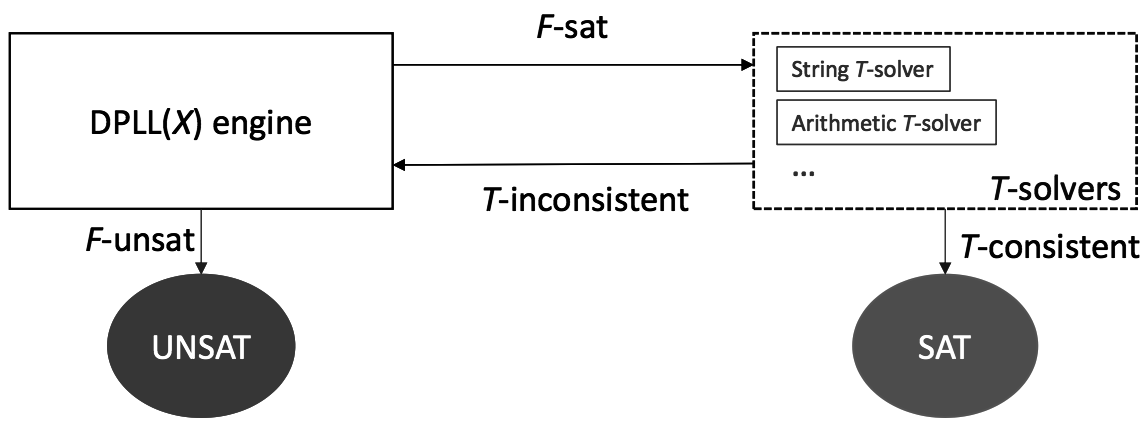
\includegraphics[width=0.8\linewidth]{pictures/dpll_arc.png}
	\end{center}
	\caption{An overview of the interaction between SAT core and $\mathcal{T}$-solvers. The image is sourced from \cite{main_phd}.}
	\label{fig:dpll_architecture}
\end{figure}

The SMT problem solving procedure  can be divided into two parts, as shown in Figure \ref{fig:dpll_architecture} : the logic solving part and the theory solving part. In the logic solving part, it usually refers to the DPLL-based SAT solver with  the capability to handle incremental clause assertions. The theory solving part usually contains several dedicated solvers for background theories. 

Initially, the SAT solver gets the formula as input. It tries to find a model for the literals. If fails, it returns $\texttt{unsat}$; otherwise, it distributes each literal to a corresponding $\mathcal{T}$-solver according to the signature of the literal.

When a $\mathcal{T}$-solver gets a set of literals, it first checks whether these literals are consistent with the theory. If it is $\mathcal{T}$-consistent, the $\mathcal{T}$-solver does nothing but reports consistent back to the SAT core. Otherwise, it either returns a conflict, or propagates a new literal. For example,  in case of our example, when the partial model $\{ s_1 ,\ s_2 ,\ s_4, \ s_5 \}$ is given to the $\mathcal{T}_{SL}$-solver. It finds a  contraction $s_1 \wedge s_2 \to \neg s_4$ and reports back to the core. 

If all $\mathcal{T}$-solvers report $\mathcal{T}$-consistent, the procedure stops and answers $\texttt{sat}$ with the current partial assignments as model ; otherwise, the SAT solver collects all clauses returned by $\mathcal{T}$-solvers, and asserts them into the formula. Then, it tries to build a model from this new formula. For example,  in case of our example, the core add $\neg s_2$ as a new fact and starts over again.